% !TEX root = ../dissertation.tex

% For VIM to recognize the document syntax \begin{document} and \end{document}
% - However, the compilation will fail!! So don't forget to comment the
%   directives before compiling!!'

%\begin{document}

% CHAPTER - Introduction -------------------------
\chapter{Introduction}

% To correctly add a marginpar, \mbox needs to be added and a blank line is also
% needed
%\ifdef{\comm}{\mbox{}\marginpar{Intro}}
%
%One of the ultimate goals of engineering is the ability to provide sustained 
%development, by efficiently using the available resources --- materials, energy,
%knowledge, time. This is a ``Sisyphus's stone''\footnote{King of Ephyra,
%condemned to push a stone uphill for eternity --- immortalised in ``The Myth of
%Sisyphus'' by Albert Camus}, a perpetual quest for optimisation of efforts and
%resources. One such example in the engineering field is the ability to produce
%components with the minimum amount of material needed for its function, i.e.,
%functional design of components without restrictions to geometry or type and
%number of different materials; instead the focus should be on the desired
%properties of such components, customising them for the specific field of
%application. 

\section{Product concept}%
\label{sec:product-concept}
\section{Product concept}%
\label{sec:orge7b0dc6}
The envisioned product consists of a remote controlled car used to assist
exploration and maintenance domains, hereby, denominated as Radio Frequency
Camera Assisted Rover (RFCAR). To satisfy such requirements, the vehicle must
contain a remotely operated camera that provides a live video feed to the user.
Additionally, the vehicle must include an odometric system that assists the
driving and avoids unintentional collisions when remote control is compromised, e.g., when connection is lost.
The vehicle provides means for exploration and conditions assessment in critical
or unaccessible areas to human operators, such as fluid pipelines and other hazardous locations.
%
%%% Local Variables:
%%% mode: latex
%%% TeX-master: "../Phase1"
%%% End:

%
%\begin{document}
\section{Context}
The functional design of components is a complex topic, with a myriad of
questions to be answered: what is the function of the component?; what design
criteria must be met to fulfil its function?; how will the component be
produced, and what data does it require?; how will the component's performance
be measured?, among others. The answers are often not clear or simple as they
dictate the use of several materials and several manufacturing technologies,
increasing severely the complexity of producing such components: how to
effectively combine two or more materials into a single component in a
synergistic way?

%%% Local Variables:
%%% mode: latex
%%% TeX-master: "../../../dissertation"
%%% End:

%\begin{document}
\section{Motivation and Goals}
The main goal of this project is to develop a remote controlled vehicle with the
following characteristics:
\begin{enumerate}
  \item Remotely operated: the vehicle must be remotely operated to enable its
    usage in critical or unaccessible areas to human operators;
  \item Provide visual feedback to the user: to be a valuable asset in the
    exploration and maintenance domains, the vehicle must provide visual
    feedback to the user of its surroundings.
  \item Safe: the vehicle must be safe to use and prevent its damage and of its
    surroundings
  \item Robust: the vehicle must be able to sustain harsh environmental
    conditions and provide redundant mechanisms to avoid control loss.
  \item Affordable: so it can be an economically viable product.
  \end{enumerate}
%%% Local Variables:
%%% mode: latex
%%% TeX-master: "../../../dissertation"
%%% End:

%\begin{document}
\section{Main objectives}
The goal of the present work is to close the gap between design and fabrication of
multi-material components from metallic/ceramic materials using
\gls{sls}/\gls{slm} technology. To this end several main objectives have been
outlined:
\begin{enumerate}
  \item Develop a design methodology for multi-material fabrication of
    metals/ceramics;
  \item Instantiate a practical workflow and respective toolchain from the
    design methodology;
  \item Develop and build a proof-of-concept equipment capable of producing
    such components;
  \item Test the production of multi-material components using the proposed
    workflow/toolchain and the equipment built.
  \end{enumerate}

  This is \gls{pi}
  
  This is \gls{omega}
%%% Local Variables:
%%% mode: latex
%%% TeX-master: "../../../dissertation"
%%% End:

% Planning
\section{Planning}%
\label{sec:planning}
%\section{Planning}%
%\label{sec:orga82318d}
In fig.~\ref{fig:gantt-diag-orig} is illustrated the Gantt chart for the project, containing the tasks' descriptions. It should be noted
that the project tasks of Analysis, Design, Implementation and Tests are
performed in two distinct iterations as corresponding to the Waterfall project
methodology.

Due to unpredictable circumstances, limiting the mobility of team
staff and goods, the implementation stage will not be done at full extent, but
rather at a simulation stage. Thus, to overcome these constraints, the project
focus is shifted to the simulation stage, where an extensive framework as to
built to model the system operation, test it, and providing valuable feedback
for the dependents modules. As an example, the modules previously connected just
by an RS232 link, must now include upstream a web module (TCP/IP) --- the data
is now effectively sent through the internet, and must be unpacked and delivery
serially as expected if only the RS232 link was used.

The tasks are described as follows:
\begin{itemize}
\item \uline{Project Kick-off}: in the project kick-off, the group is formed and the tutor
is chosen. A brainstorming about conceivable devices takes place, whose
viability is then assessed, resulting in the product concept definition
(Milestone 0).
\item \uline{State of the Art}: in this stage, the working principle of the device is
studied based on similar products and the system components and its
characteristics are identified.
\item \uline{Analysis}: In the first stage --- Analysis 1 --- contains the analysis
results of the state of the art. It should yield the specifications document,
containing the requisites and restrictions to the project/product, on a
quantifiable basis as required to initiate the design; for example, the
vehicle's desired speed should be, at maximum, \texttt{2 m/s}. The second stage --- Analysis 2
--- contains the analysis of the first iteration of the development cycle.
\item \uline{Design}: it is done in two segments: modules design --- where the modules are
designed; integration design --- where the interconnections between modules is
designed. It can be subdivided into \emph{conceptual design} and \emph{solution
design}. 
\begin{itemize}
\item In the conceptual design, several problem solutions are identified,
quantifying its relevance for the project through a measuring scale,
inserted into an evaluation matrix, for example, QFD.%
\item In the solution design, the selected solution is developed. It must include
the solution modelling, e.g.:
\begin{itemize}
\item \uline{Control system}: analytically and using simulation;
\item \underline{Transducer design}: circuit design and simulation;
\item \uline{Power system}: power supply, motors actuation and
  respective circuitry design and simulation;
\item \uline{Communications middleware}: communication protocols evaluation and
  selection;
\item \uline{Software layers}: for all required modules, and considering its
  interconnections, at distinct levels:
  \begin{itemize}
  \item \uline{front end layer}: user interface software, providing a easy and convenient
    way for the user to control and manage the system.
  \item \uline{framework layer}: software required to emulate/simulate and test the
    required system behaviour, providing seamless interfaces for the dependents
    modules
  \item \uline{back end layer}: software running \emph{behind the scenes}, handling user
    commands received, system monitoring and control.
  \end{itemize}
\end{itemize}
\end{itemize}
\item \uline{Implementation}: product implementation which is done by
  \uline{modular integration}. In the first stage, the implementation is done in a prototyping
environment --- the assisting framework developed, yielding version alpha; in the second stage
it must include the coding on the final target modules, yielding
prototype beta.
\item \uline{Tests}: modular tests and integrated tests are performed. Tests are generally considered as those performed over any physical
component or prototype. Here, it is used as a broader term, to reflect the tests
conducted into the system and the several prototypes.
\item \uline{Functional Verification/Validation}: System verification may be performed to validate overall
  function, but not for quantifiable measurement, due to the latencies
  involved. Regarding validation, specially for an external agent, thus, it should be limited
  to user interface validation.
\item \uline{Delivery}: --- project closure encompassing:
\begin{enumerate}
\item Final prototype
\item Support documentation: how to replicate, instruction manual.
\item Final report
\item Public presentation
\end{enumerate}
\end{itemize}
%
%%%%%%%%%%%%%%% Figure is deprecated: use PDF instead
%\begin{figure}[!htbp]
%\centering
%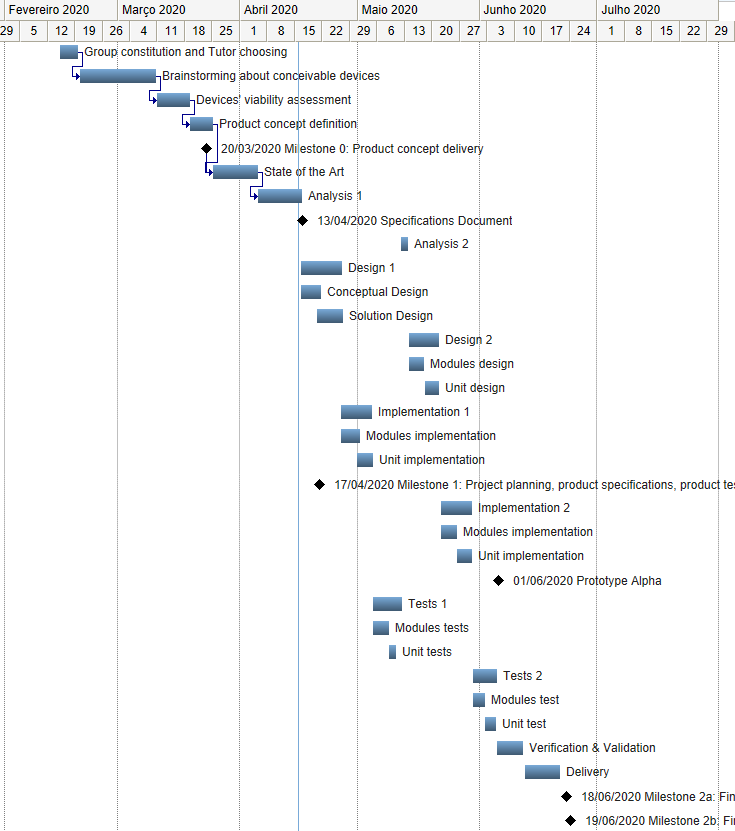
\includegraphics[width=1.0\textwidth]{./sec/img/gantt-diag-orig.png}
%\caption{\label{fig:gantt-diag2}Project planning: Gantt diagram 1}
%\end{figure}
%\begin{figure}[!htbp]
%\centering
%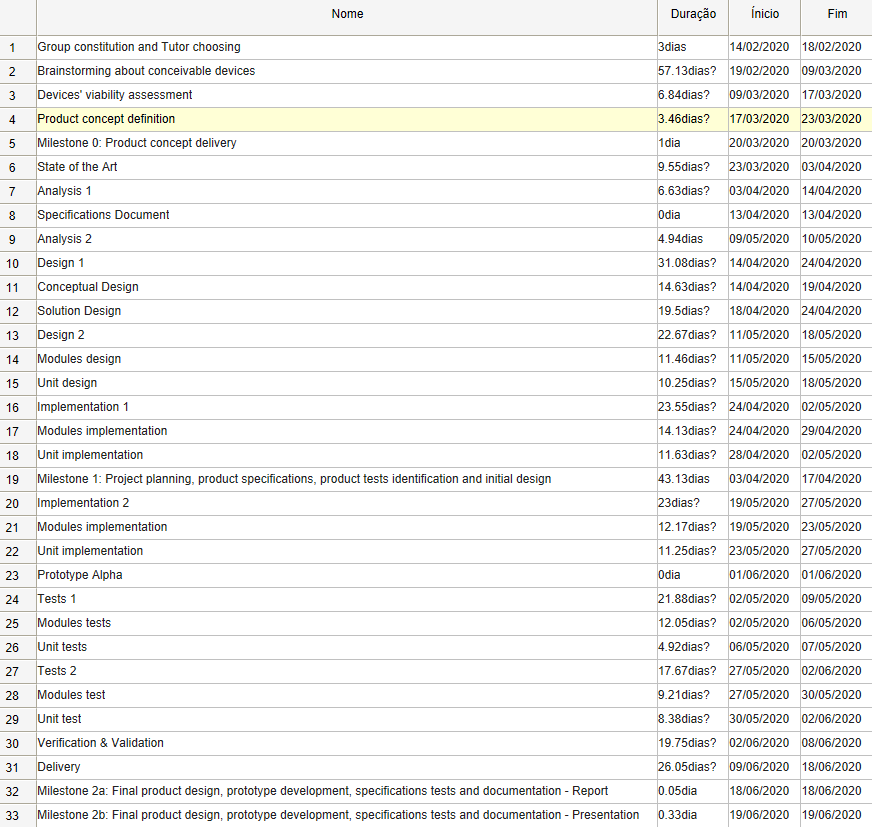
\includegraphics[width=1.0\textwidth]{./sec/img/gantt-orig-tasks.png}
%\caption{\label{fig:gantt-tasks}Project planning: tasks}
% \end{figure}
%%%%%%%%%%%%%%%%%%%%%%%%%%%%%%%%%%%%%%%%%%%%%%%%%%%%%%%%%%%%%
% 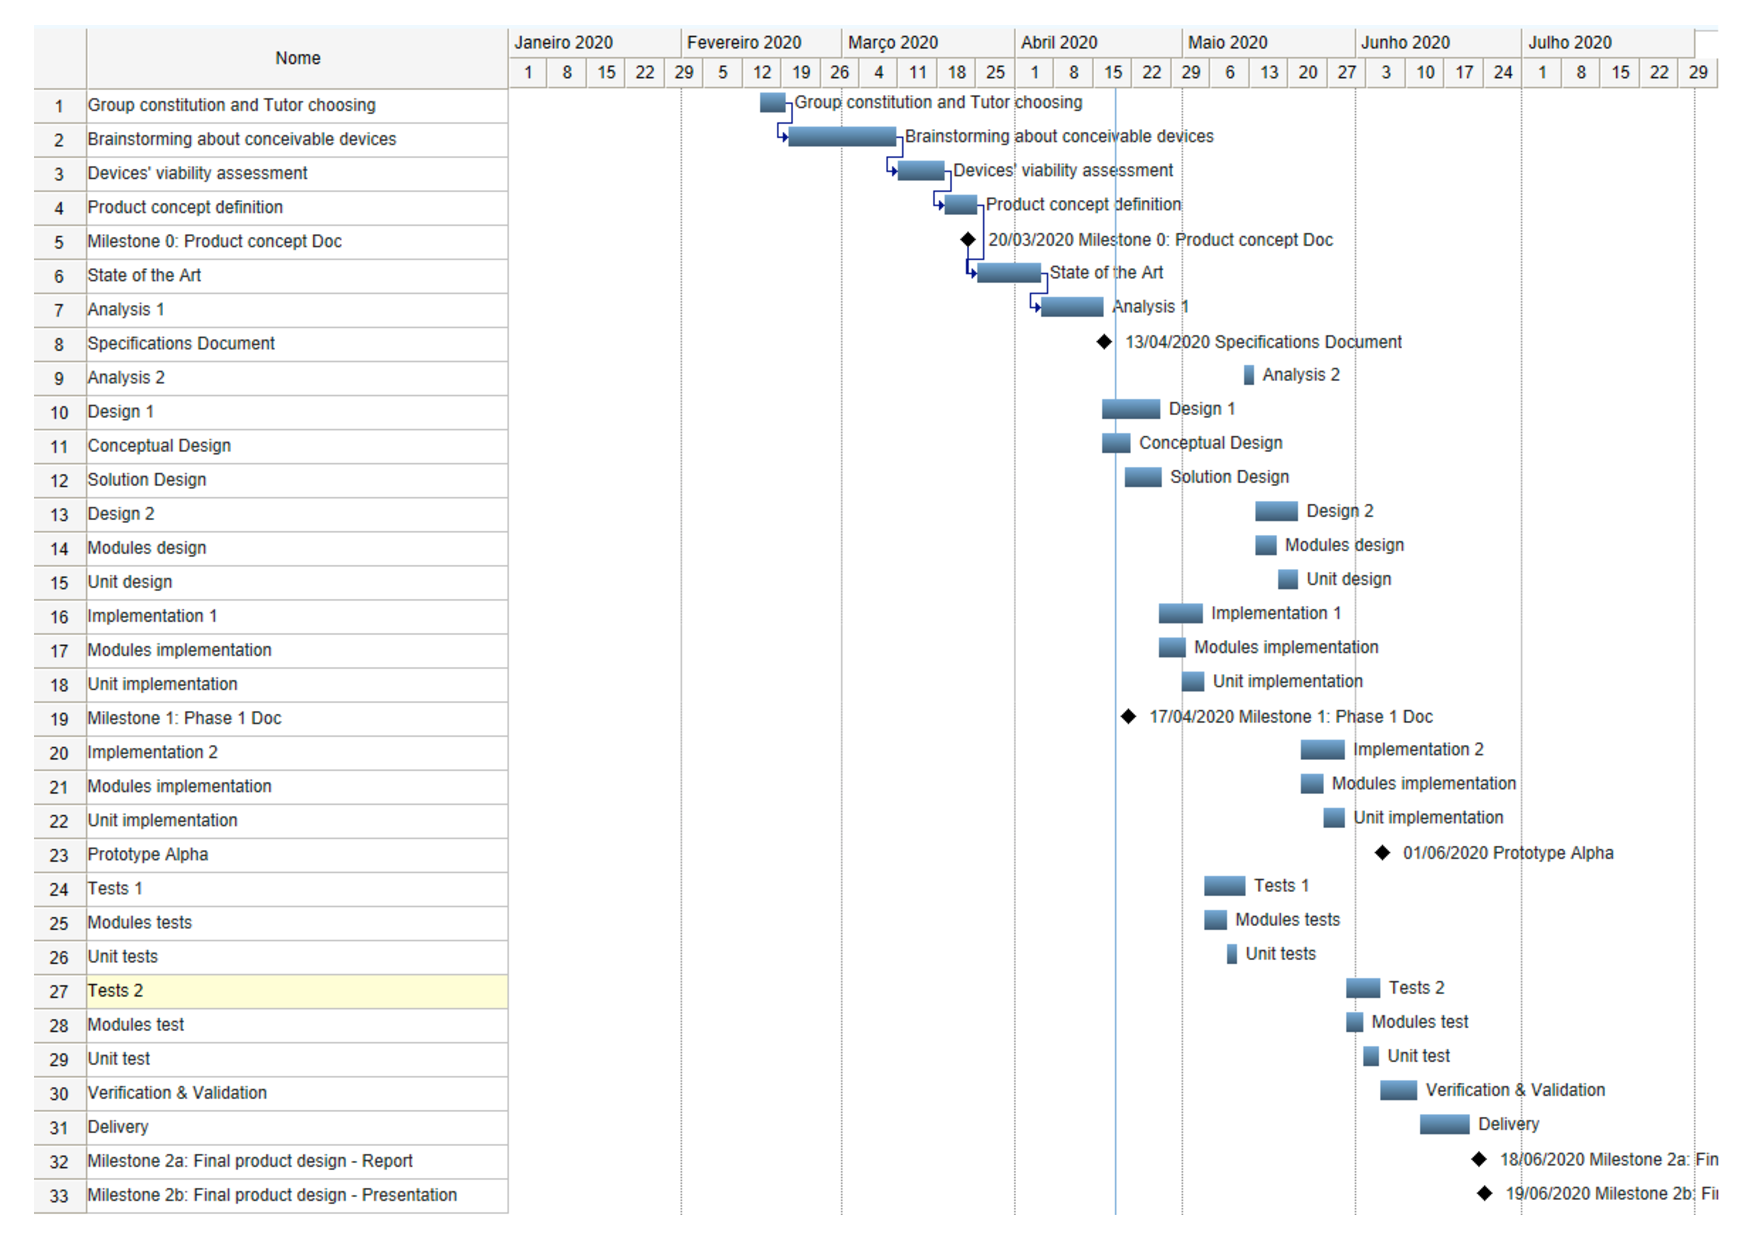
\includepdf[pages=-]{sec/pdf/gantt-diag-orig.pdf}
\begin{sidewaysfigure}[!h]
  \centering
  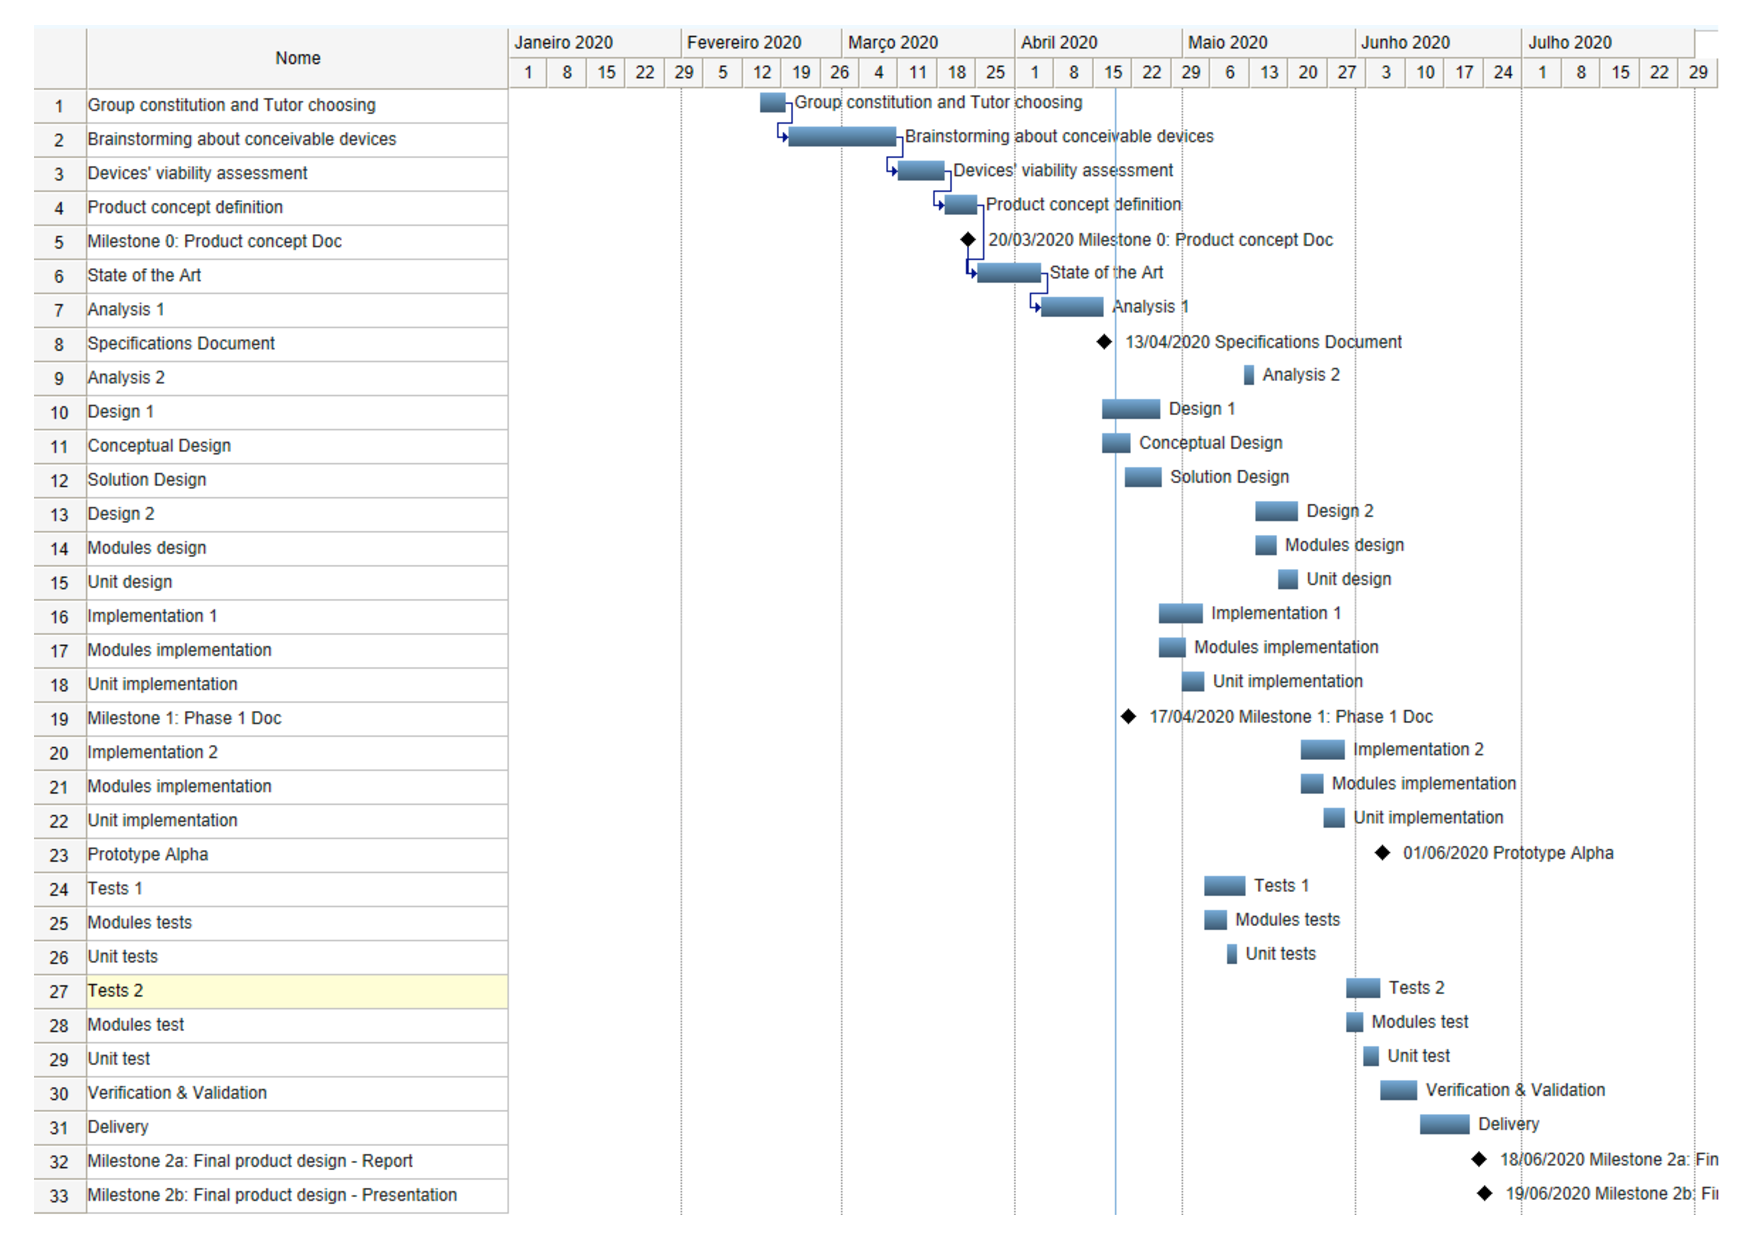
\includegraphics[page=1,width=1.0\textwidth]{sec/pdf/gantt-diag-orig.pdf} 
  \caption{Project planning --- Gantt diagram}%
  \label{fig:gantt-diag-orig}
\end{sidewaysfigure}
% 
%%% Local Variables:
%%% mode: latex
%%% TeX-master: "../Phase1"
%%% End:

%
\section{Research hypothesis (optional)}

  Reseach hypothesis


%\begin{document}
\section{Report organisation}
This report is organised as follows:
In Chapter~\ref{ch:state-art}, the state of the art of the additive
manufacturing technology, \gls{lbam}, and \gls{mmam} is presented, with special
focus on the last, namely on \gls{fgm} structures. Lastly, a brief overview of
the available methodologies in these fields are presented.

In Chapter~\ref{ch:theor-found} the theoretical foundations are presented, namely the project development methodologies and associated tools,
and the \gls{sls}/\gls{slm} process in detail.

In Chapter~\ref{ch:prob-challenge}, the multi-material design and production
problem and its challenges using \gls{sls}/\gls{slm} technology are
presented. The methodology devised for multi-material production through the
\gls{lbam} technology is presented to tackle the high complexity of the process
and the lack of a supporting methodology, taking into account the key agents of
the process and leveraging the process information.

In Chapter~\ref{ch:development} is presented all the development phase of the
project. A specific workflow was instantiated from
the methodology, attending to the specific requirements and constraints of the
project. Based on this workflow, a toolchain was assembled, designing the
required software components. Finally, based on the requirements and constraints
of the process itself, the mechanical and electronic infrastructures were
designed, and on top of the last, the control software was designed.

In Chapter~\ref{ch:application}, the workflow and equipment were put to the test
to verify their suitability to the process and their performance for
multi-material component production. Additionally, production manufacturing tests
were also performed. Tests were used to validate the workflow and equipment,
pointing out also straightforward ways to adapt and implement custom paths for
the multi-material \gls{lbam} process.

The Chapter~\ref{ch:conclusion} gives a summary of this thesis as well as
prospect for future work.

Lastly, the appendices (see Section~\ref{ch:Append}) contain detailed information...
%%% Local Variables:
%%% mode: latex
%%% TeX-master: "../../../dissertation"
%%% End:

%
%%% Local Variables:
%%% mode: latex
%%% TeX-master: "../../../dissertation"
%%% End:
